




%%%
%%% This document is now read-only and reflects the version sent to IMPACT.
%%%






\documentclass[sigplan]{acmart}
\usepackage[utf8]{inputenc}
\usepackage{xargs}
\usepackage[textsize=scriptsize,textwidth=1.5in]{todonotes}
\usepackage{listings}
\usepackage{minted}
\usepackage[outline]{contour}% http://ctan.org/pkg/contour
\usepackage{xspace}
\usepackage{amsmath}
\usepackage{color, colortbl}

% Uncomment me for the final version.
\def\finalversion

\ifthenelse{\isundefined{\finalversion}}{
\addtolength{\marginparwidth}{1in}
\addtolength{\hoffset}{0.8in}
\addtolength{\paperwidth}{2in}

\newcommandx{\az}[2][1=]{\todo[linecolor=blue,backgroundcolor=blue!25,bordercolor=blue,#1]{\textbf{Alex:} #2}}
\newcommandx{\wmnote}[2][1=]{\todo[linecolor=blue,backgroundcolor=blue!25,bordercolor=blue,#1]{\textbf{Billy:} #2}}
\newcommandx{\rz}[2][1=]{\todo[linecolor=blue,backgroundcolor=blue!25,bordercolor=blue,#1]{\textbf{Ruizhe:} #2}}
\newcommandx{\lc}[2][1=]{\todo[linecolor=blue,backgroundcolor=blue!25,bordercolor=blue,#1]{\textbf{Lorenzo:} #2}}
}{
\renewcommand{\todo}[2]{}
\newcommandx{\wmnote}[2][1=]{}
\newcommandx{\az}[2][1=]{}
\newcommandx{\rz}[2][1=]{}
}


\newcommand{\icode}[1]{{\texttt {#1}}}
\newcommand{\tool}{Polygeist\xspace}
\newcommand{\memref}{\icode{memref}\xspace}
\newcommand{\scop}{SCoP\xspace}
\newcommand{\polycc}{\icode{polycc}\xspace}

\tikzset{
  cfedge/.style={
    font=\itshape,
    draw=black,
    ->,
    >=stealth'
  },
  process/.style={
    draw,
    fill=orange!50,
    rectangle,
    minimum height=1.5em,
    minimum width=6em,
    align=center,
    font=\small,
  }
}

\lstset{basicstyle=\ttfamily}

\lstdefinelanguage{llvm}{
	% see https://tex.stackexchange.com/questions/137237/listings-text-highlighting-based-on-prefix
    %moredelim=[s][\color{orange3}]{x}{>},
    alsoletter={\%,\#,!},
    keywordsprefix={\%},
    morekeywords={\%},
    keywordstyle=\color{orange3},
    % this allows to color inside <memrefxf32> (i.e., f32).
    otherkeywords={index, f32, i32, f64, i8},
    keywords=[3]{index, f32, memref, i32, f64, i8, affine_map, affine_set},
    keywordstyle=[3]\color{scarletred3},
    showstringspaces=false,
	breaklines=true,
    breakatwhitespace=true,
    morestring=[b]",
    stringstyle=\color{green3},
    moredelim=[s][\color{blue3}]{\#}{<},
    moredelim=[s][\color{scarletred3}]{!}{\ },
}


\newcommand{\midsepremove}{\aboverulesep = 0mm \belowrulesep = 0mm}
\definecolor{orange3}{rgb}{0.808,0.361,0.000}
\definecolor{scarletred3}{rgb}{0.643,0.000,0.000}
\definecolor{green3}{rgb}{0.000,0.405,0.000}
\definecolor{blue3}{rgb}{0.000,0.000,0.704}
\definecolor{aluminium1}{rgb}{0.933,0.933,0.925}
\definecolor{aluminium2}{rgb}{0.827,0.843,0.812}
\definecolor{aluminium3}{rgb}{0.729,0.741,0.714}
\definecolor{aluminium4}{rgb}{0.533,0.541,0.522}
\definecolor{aluminium5}{rgb}{0.333,0.341,0.325}
\definecolor{aluminium6}{rgb}{0.180,0.204,0.212}

% \wmnote{Misc trying to name}
% C++

% MLPT: Multi-Level Polyhedral Tool

% Fair 

% RACPM: Raising C++ to Polyhedral MLIR

% Connecting MLIR C++ and Polyhedral Tools With C++
% Connecting MLIR C++ and Polyhedral Tools
% Frontend
% Connecting 
% Translating
% Compiling     
% Extracting MLIR for polyhedral research from MLIR

% Evaluating Polyhedral tools on C++MLIR

% Polyhedral MLIR extraction from C++

% AMT PolyC++ - : Affine MLIR Tools from Polyhedral C++

% PolyCAM Polyhedral C to Affine MLIR

% Making MLIR

% CRIMPT: C++ Lowering in MLIR Polyhedral Tool
% CRIMPT: C++ Raising in MLIR Polyhedral Tool

% CRIM 

% Fair Ablation Analysis by Bringing  
% C++
% Compiler/ing
% Polyhedral
% MLIR

% Infrastructure Representation
% Fair
% Ablation
% Making
% Bringing
% Tools

% ccoplmir

% cpmlir
% pomcc
%\title{Affine C in MLIR}
\title{Polygeist: Affine C in MLIR}
%\title{Polygeist: Raising C to Polyhedral MLIR}
% RZ: no capitalization for Into and The?
%\subtitle{Bringing Polyhedral Tools Into The MLIR Infrastructure}
\date{November 2020}

\author{William S. Moses}
\affiliation{
 \institution{MIT CSAIL}
 \country{}}
\email{wmoses@mit.edu}

\author{Lorenzo Chelini}
\affiliation{
  \institution{TU Eindhoven}
  \country{}}
\email{l.chelini@tue.nl}

\author{Ruizhe Zhao}
\affiliation{
  \institution{Imperial College London}
  \country{}}
\email{ruizhe.zhao15@imperial.ac.uk}

\author{Oleksandr Zinenko}
\affiliation{
  \institution{Google}
  \country{}}
\email{zinenko@google.com}

\settopmatter{printfolios=true,printccs=false,printacmref=false}
\acmConference[IMPACT 2021]{11th International Workshop on Polyhedral
Compilation Techniques - in conjunction with HiPEAC 2021}{January 20,
2021}{Budapest, Hungary}
\setcopyright{none}
\copyrightyear{\?}
\def\?#1{}
\acmDOI{}
\acmPrice{}
\acmISBN{}


\begin{abstract}
We present \tool, a new tool that reroutes polyhedral compilation flows to use the representation available in the recent MLIR compilation infrastructure. It consists of two parts: a C and C++ frontend capable of converting a wide variety of existing codes into MLIR suitable for polyhedral transformation, and a bi-directional conversion between MLIR's polyhedral representation and existing polyhedral exchange formats. We demonstrate \tool's flow by converting the entire Polybench/C benchmark suite into MLIR, and by performing an IR-to-IR optimization leveraging an existing polyhedral compiler (Pluto). Our flow produces results within 1.25\% of the state-of-the-art Clang compiler, enabling direct comparison of source-to-source and IR-to-binary compilers.
%% Discuss Polymer numbers?
%% If we want to include parallel numbers here, but I feel it detracts from the story a bit
We believe \tool can improve the interoperation between MLIR and the existing polyhedral tooling, benefiting both the research and the production compiler communities.

\end{abstract}

\begin{document}

\maketitle

\section{Introduction}
The polyhedral model has remained on the cutting edge of research into compiler optimizations for several decades~\cite{feautrier2011polyhedron}.
It provides deep loop analysis and restructuring capabilities by transforming the input program into a mathematical abstraction based on integer sets and binary relations, reasoning on this abstraction and generating the new, optimized code.
The process of transforming the program from the representations commonly used in production compilers such as LLVM intermediate representation (IR)~\cite{llvm} or syntax tree is non-trivial~\cite{grosser.ppl.2012,pop2006graphite}, and the inverse process is even more complex~\cite{cloog,razanajato2017splitting,grosser2015polyhedral}.
This process, together with high algorithmic complexity of the underlying transformation mechanism, has led to the polyhedral optimization being rather poorly adopted by compilers beyond research.

MLIR is a new compiler infrastructure proposed and developed in the scope of the LLVM project~\cite{mlir}.
One of its design goals is to provide a production-grade infrastructure that simplifies the expression of advanced compiler optimization, in particular those that require to cast the input program into an additional, higher-level abstraction.
Given the growing evidence that the polyhedral model is one of the best frameworks for efficient transformation of machine learning programs~\cite{tc,teckyl,mullapudi2015polymage} and is particularly well suited for existing and emerging accelerator architectures~\cite{cerebras_chip,ppcg,tc_cim}, MLIR has always considered the polyhedral representation as a first-class citizen in its infrastructure~\cite{mlir_rationale}.
Its approach to polyhedral optimization attempts to address the complexity and comprehensibility issues by designing and implementing all relevant algorithms from scratch, and by using a simplified representation that updates the code after each transformation instead of relying on a monolithic code generation mechanism~\cite{mlir_simplified_polyhedral}.

The design of MLIR's affine representation~\cite{mlir_affine} makes it challenging to directly apply existing polyhedral tools, which are often based on \icode{isl}~\cite{isl} or \icode{Polylib}~\cite{polylib} and designed for C source-to-source transformation~\cite{Bondhugula2008Pluto,ppcg}. Additionally, benchmarks used in the literature on polyhedral compilation are commonly written in C~\cite{polybench} and are not benefiting from the higher level representations available in MLIR~\cite{linalg}. As a result, empirical comparisons can only be performed for the entire end-to-end compilation flows, and it is difficult to identify to which extent each part of the flow (high-level representation, polyhedral transformation, post-polyhedral downstream compiler) affects the final performance. 

We address these issues in two ways. First, we create a compilation flow that connects MLIR polyhedral representation to existing tools such as Pluto~\cite{Bondhugula2008Pluto} and CLooG~\cite{cloog}. Our bi-directional conversion between the MLIR Affine dialect~\cite{mlir_affine} representation and the OpenScop format~\cite{openscop} allows developers to build flows that originate in MLIR, use existing polyhedral tools, and return to MLIR for further transformation and executable code generation. Second, we create a \icode{Clang}-based C and C++ MLIR frontend capable of identifying static control parts of the program (\scop) to produce the Affine dialect along with other ``standard'' MLIR dialects. This enables MLIR flows to compile common polyhedral benchmarks as well as other code bases written in C or C++ without rewriting them in a different input language.

Bringing both standard tools and benchmarks to MLIR provides researchers with several benefits. Notably, this enables ablation analysis of the benefits of a given MLIR-based polyhedral transformation and the use of existing polyhedral tools to optimize MLIR inputs (rather than C or C++ inputs). While this naturally opens up the door for creating and evaluating new transformations, in this work, we \emph{only} consider the effectiveness of our \tool workflow. More specifically, we demonstrate that \tool is able to process the benchmarks of interest without significant overhead, and that MLIR transformations compose with existing polyhedral flows.
%nor does it provide any unexplained advantage (or disadvantage) to the MLIR-based flow, with and without polyhedral transformations.
%This work will enable more precise comparisons of polyhedral compilation flows across different infrastructures.

\section{Background: MLIR Framework}
\subsection{Overview}
MLIR is an optimizing compiler infrastructure inspired by LLVM~\cite{llvm} with focus on extensibility and modularity~\cite{mlir}.
It is based on the principles of concept parsimony (the IR has as little built-in concepts as possible), effect traceability (the provenance of any IR construct can be traced back to some location in the input program) and transformation progressivity (optimizations are performed in incremental, verifiable steps that maintain the validity of the IR).

Practically, MLIR defines an SSA-based~\cite{ssa} IR and provides algorithms and tools to analyze and transform it.
Like many SSA representations, MLIR uses \emph{values} as a unit of data processed by the represented program.
MLIR values cannot be redefined.
The actions of a program are described using \emph{operations}, which can be seen as a generalization of (machine) instructions or high-abstraction operations such as matmul, that use values and define new values.
Operations are the main mechanism for defining the semantics of the program.
Values in MLIR have a \emph{type}, which contains the information known about the value at compile time.
Similarly, operation \emph{attributes} contain the additional information about the operation known at compile time.
Operations are organized into linear sequences of (basic) \emph{blocks} that are executed sequentially.
Blocks may accept values as arguments, following the functional SSA form~\cite{appel1998ssa} as opposed to the $\phi$-node form.
Groups of blocks are in turn collected into \emph{regions}.
MLIR supports regions with classical control flow graph (CFG) structure where the control can flow from one block to one of its \emph{successors} as well as arbitrary graph regions that can have custom semantics such as TensorFlow graphs.
We only consider CFG regions throughout this paper.
Regions can be attached to an operation, which defines how the control flows into and from these regions, allowing the IR to be arbitrarily nested at multiple levels.
MLIR supports polyhedral analysis by providing attributes for \emph{integer sets} and \emph{affine maps}, described in more detail in Section \ref{sec:affine}.
The generic syntax, accepted by all operations, is illustrated in Figure~\ref{fig:mlir_syntax}.
Additionally, MLIR allows attributes, operations, and types to define custom syntax.

\begin{figure}
{
\scriptsize
\begin{lstlisting}[language=llvm,escapeinside=@@, mathescape=true]
%result = "dialect.operation"(%operand, %operand)
          {attribute = #dialect<"value">} ({
^basic_block(%block_argument: !dialect.type):
  "another.operation"() : () -> ()
}) : (!dialect.type) -> !dialect.result_type
\end{lstlisting}
}
\caption{Generic MLIR syntax for an operation with two operands, one result, one attribute and a single-block region.}
\label{fig:mlir_syntax}
\end{figure}

The key power of MLIR resides in its extensibility: its only built-in concepts are attributes, types, operations and regions described above.
For example, modules and functions \emph{need not} be a first-class concept in MLIR and are instead defined as operations with specific semantics, ``symbol name'' attributes, and a region to represent their body.
In the same spirit, MLIR allows one to define operations ranging from high-level constructs such as ``for'' loops or functional ``map/reduce'' to low-level hardware instructions, and even hardware itself~\cite{circt}.

Attributes, operations and types that are expected to be used together are organized in \emph{dialects}, which can be thought of as modular dynamic libraries.
MLIR provides a handful of dialects that define common operations such as modules, functions, loops, memory or arithmetic instructions as well as ubiquitous types such as integers, floats, and tuples.

\subsection{Affine Dialect}\label{sec:affine}
The \emph{Affine} dialect is one of the first dialects created in the MLIR project~\cite{mlir_affine}.
It is intended for representing \scop's with explicit polyhedral-friendly loop and conditional constructs.
The core of its representation is the following classification of value categories:
\begin{itemize}
    \item \emph{Symbols}---integer values that are known to be loop-invariant but unknown at compile time, also referred to as program \emph{parameters} in polyhedral literature, typically array dimensions or function arguments. In MLIR, symbols are values defined in the top-level region of an operation with ``affine scope'' semantics, e.g. functions; or array dimensions, constants and results of affine map application regardless of their definition point.
    \item \emph{Dimensions}---are an extension of symbols that also accepts induction variables of affine loops.
    \item \emph{Non-affine}---any other values.
\end{itemize}
Symbols and dimensions have \icode{index} type, which is a platform-specific integer that fits a pointer (i.e., \icode{intptr\_t} in C).

\emph{Affine maps} are multi-dimensional (quasi-)linear functions of a list of dimension and symbol arguments.
For example, $(d_0, d_1, d_2, s_0) \rightarrow (d_0 + d_1, s_0 \cdot d_2)$ is a two-dimensional quasi-affine map from three dimensions and one symbol.
The same map in MLIR syntax is \icode{affine\_map<(d0, d1, d2)[s0] -> (d0 + d1, s0 * d2)>}.
The affine map construct does \emph{not} require its arguments to have the symbol and dimension category, only \emph{some} operations in the affine dialect do.
Instead, the separation between dimensions and symbols allows for quasi-linear expressions: symbols are treated as constants and can therefore be multiplied with dimensions whereas a product of two dimensions is invalid.

\emph{Integer sets} are collections of integer tuples that are constrained by a conjunction of (quasi-)linear expressions.
For example, a ``triangular'' set $\{(d_0, d_1) : 0 \leq d_0 < s_0 \land 0 \leq d_1 \leq d_0\}$ can be expressed as
\icode{affine\_set<(d0, d1)[s0] : (d0 >= 0, s0 - d0 - 1 >= 0, d1 >= 0, d0 - d1 >= 0)>}.

The Affine dialect makes use of the concepts above to define a set of operations.
An \icode{affine.for} is a ``for'' loop with lower and upper bounds expressed as affine maps of symbol and dimension values, and a constant step.
The bounds are computed when the loop is about to be executed and are loop-invariant.
If the affine maps are multidimensional, a \icode{max} (\icode{min}) of the results defines the lower (upper) bound.
The region is a single block that corresponds to the body of the loop and takes the induction variable as loop argument.
An \icode{affine.parallel} is a ``multifor'' loop nest, iterations of which can be executed concurrently.
An \icode{affine.if} is a conditional construct, with an optional \icode{else} region, and a condition defined as inclusion of the given dimension and symbol values into an integer set.
Finally, \icode{affine.load} and \icode{affine.store} are used to express memory accesses where the address computation is expressed as an affine map of dimensions and symbols.

\begin{figure}
{
\scriptsize
\begin{lstlisting}[language=llvm, escapeinside=@@, mathescape=true]
%c0 = constant 0 : index
%0 = dim %A, %c0 : memref<?xf32>
%1 = dim %B, %c0 : memref<?xf32>
affine.for %i = 0 to affine_map<()[s0] -> (s0)>()[%0] {
  affine.for %j = 0 to affine_map<()[s0] -> (s0)>()[%1] {
    %2 = affine.load %A[%i] : memref<?xf32>
    %3 = affine.load %B[%j] : memref<?xf32>
    %4 = mulf %2, %3 : f32
    %5 = affine.load %C[%i + %j] : memref<?xf32>
    %6 = addf %4, %5 : f32
    affine.store %6, %C[%i + %j] : memref<?xf32>
  }
}
\end{lstlisting}
}
\vspace{-.5cm}
\caption{Polynomial multiplication in MLIR using Affine and Standard dialects.}
\label{fig:polynomial}
\end{figure}

Figure~\ref{fig:polynomial} illustrates the Affine dialect by using it to define a polynomial multiplication, \icode{C[i+j] += A[i] * B[j]}.
Operations not prefixed with \icode{affine.} are defined in the Standard dialect and correspond to common instructions.
Even such a simple example highlights the fact that MLIR supports, and encourages, IRs from different dialects to be used together.

\subsection{Memory References}\label{sec:memref}

\begin{figure}
    \centering
    \includegraphics[width=0.7\columnwidth]{images/memref.png}
    \vspace{-.5cm}
    \caption{MLIR supports multi-dimensional memory references indexed with affine maps.}
    \label{fig:memref}
\end{figure}

Figure~\ref{fig:polynomial} also makes use of a core MLIR type---\memref, which stands for \textbf{\texttt{mem}}ory \textbf{\texttt{ref}}erence.
It is a structured multi-index pointer into memory that does not allow internal aliasing, i.e., different indices always point to different addresses.
This effectively defines away the delinearization problem that hinders the application of polyhedral techniques at the LLVM IR level~\cite{delinearization}.
By default, {\memref}s are expected to have a \emph{strided} format similar to the one used for tensors in machine learning framework.
A strided \memref is described by its \emph{rank}, \emph{offset} from the base pointer, a list of \emph{sizes} and a list of \emph{strides}.
The latter indicates the number of elements one needs to skip to obtain the next element along a dimension.
Strides can thus express various layouts.
For example, an $M \times N$ \memref with strides $N, 1$ is row-major, with strides $1, M$ is column-major, while the strides $2N$ and $2$ combined with $\mathrm{offset}=1$ define a layout accessing odd columns in even lines as illustrated in Figure~\ref{fig:memref}.
In general, the list of indices is transformed into the linear address as 
$A = \mathrm{base} + \mathrm{offset} + \sum_i \mathrm{stride}_i \cdot \mathrm{index}_i.$
One can observe that, for a fixed rank, this can be expressed using an affine map by treating offset and strides as symbols:
\icode{affine\_map<(i0,i1)[A,off,s0,s1] -> (A + off + \\ s0*i0 + s1*i1)>}.
This is intentional and makes {\memref}s compatible with affine transformations.

%Other, more complex affine maps can be used in \memref layouts, and they also support dynamic ranks, but such cases are irrelevant for the further discussion.

\subsection{Other Relevant Core Dialects}
MLIR  provides several dozen dialects.
Out of those, only a handful are relevant for our discussion.
The \emph{Structured Control Flow} (\icode{scf}) dialect defines the control flow operations such as loops and conditionals that are not constrained by affine categorization rules.
For example, a \icode{scf.for} loop accepts any integer value as lower bound, upper bound or step and does not support any affine maps.
The \emph{Standard} (\icode{std}) dialect contains common operations such as integer and float arithmetic, (non-affine) memory accesses or branching control flow.
It is used as a common lowering point from higher-level dialects before fanning out into multiple target dialects and can be seen as an extreme generalization of LLVM IR~\cite{llvm}.
At the same time, the \emph{LLVM} dialect provides a direct mapping of LLVM IR instructions and types into MLIR.
It is primarily used to simplify the translation process between the two representations if further processing by LLVM is necessary.
Finally, the \emph{OpenMP} dialect provides a dialect- and platform-agnostic representation of OpenMP directives such as ``parallel'' and ``workshare loop''. It can be used to emit LLVM IR interacting with an OpenMP runtime.
%\lc{remove OpenMP dialect?}
%\az{I'm still reasonably hopeful about exercising OpenMP.}

\section{An (Affine) C or C++ Frontend for MLIR}

\begin{figure*}
\begin{center}
\includegraphics[scale=0.75]{images/pipeline.pdf}
\vspace{-.3cm}
\caption{\tool flow. MLIR's SCF constructs are generated by traversing the Clang AST after the emission \tool raising passes enables emission of affine constructs.}
\label{fig:pipeline}
\end{center}
\end{figure*}

\iffalse
\begin{figure}
\centering
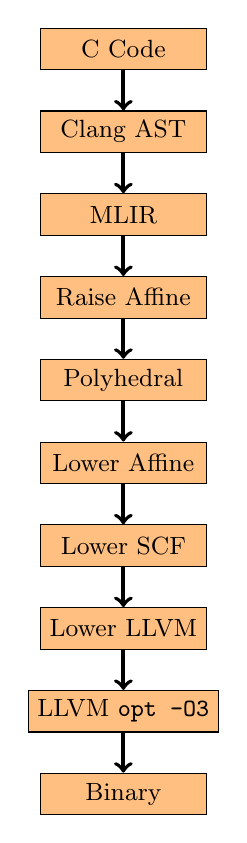
\begin{tikzpicture}[auto, node distance=.51cm and 0.6cm]

    \node [process] (clang1) {C Code};

    \node [process, below= of clang1] (opt1) {Clang AST};

    \node [process, below= of opt1] (enzyme1) {MLIR};

    \node [process, below= of enzyme1] (popt1) {Raise Affine};

    
    \node [process, below= of popt1] (clang2) {Polyhedral};

    \node [process, below= of clang2] (enzyme2) {Lower Affine};

    \node [process, below= of enzyme2] (opt2) {Lower SCF};

    \node [process, below= of opt2] (popt2) {Lower LLVM};

    \node [process, below= of popt2] (cg2) {LLVM \icode{opt -O3}};

    \node [process, below= of cg2] (cg1) {Binary};

    \draw [->, line width=0.5mm] (clang1) -- node {} (opt1);
    \draw [->, line width=0.5mm] (opt1) -- node {} (enzyme1);
    \draw [->, line width=0.5mm] (enzyme1) -- node {} (popt1);
    \draw [->, line width=0.5mm] (popt1) -- node {} (clang2);

    \draw [->, line width=0.5mm] (clang2) -- node {} (enzyme2);
    \draw [->, line width=0.5mm] (enzyme2) -- node {} (opt2);
    \draw [->, line width=0.5mm] (opt2) -- node {} (popt2);
    \draw [->, line width=0.5mm] (popt2) -- node {} (cg2);
    \draw [->, line width=0.5mm] (cg2) -- node {} (cg1);
  \end{tikzpicture}
\caption{Lowering Pipeline}
\label{fig:pipeline}
\end{figure}
\fi

Figure~\ref{fig:pipeline} shows an overview of \tool. Starting from a code fragment expressed using C or C++, \tool traverses the Clang AST and for each visited node emits the corresponding MLIR SCF or Standard dialect construct. In contrast to LLVM-based tools like Polly~\cite{grosser.ppl.2012}, \tool takes advantage of MLIR's ability to express control flow constructs such as loops directly, eliminating the need to discover loops in CFG.\footnote{Polly is still useful to discover loop constructs in code that was not originally written as explicit C or C++ loops.}
At SCF level, \tool exposes a raising pass which allows lifting Standard load, store, as well as SCF ``for'' loops and ``if'' conditions to the Affine dialect. At the Affine level, code is optimized and lowered back to SCF, which in turn, gets lowered to LLVM IR for code generation. Finally, \icode{Clang} takes LLVM IR and emits binary code, to be executed on the target platform.

\subsection{Converting \icode{Clang} AST to MLIR}
\tool leverages Clang infrastructure to perform syntactic and semantic analysis of the input code. Provided with C or C++ files and the name of the entry function, \tool lazily emits IR for each function transitively called from the entry point. \tool achieves this by traversing the AST and converting each node (``if'', ``for'', a binary operator, etc.) to an equivalent construct in MLIR's SCF or Standard dialect. This approach enables handling multi-versioned functions and allows users to, e.g., only produce IR for specific functions.

C or C++ types in the AST are first lowered to LLVM, as is done in Clang's normal compilation process, and then converted to an equivalent MLIR type in the Standard dialect (see Table~\ref{table:types}). Doing so allows \tool to generate code with a compatible Application Binary Interface (ABI) as existing compilers without re-implementing significant pieces of infrastructure. Standard library calls such as \icode{pow} are emitted as operations of the Standard dialect or declared as external functions.

\begin{table}[]
  \centering
  \resizebox{\columnwidth}{!}{%
  {\tt
  \begin{tabular}{lll}
  \toprule
  {\rm\bf C type} & {\rm\bf LLVM IR type} & {\rm\bf MLIR type} \\
  \midrule
  int & i32 (on machine X) & i32 (on machine X) \\
  intNN\_t & iNN & iNN \\
  uintNN\_t & iNN & uiNN \\
  float & float & f32 \\
  double & double & f64 \\
  ty * & ty * & memref<?\,x\,ty> \\
  ty ** & ty ** & memref<memref<?\,x\,ty>\ \!\!\!> \\
  ty[N][M] & ty[N][M] & memref<N\,x\,M\,x\,ty> \\
  \bottomrule
  \end{tabular}
  }
  }
  \caption{Type correspondence between C, LLVM IR and MLIR Standard types.}
  \label{table:types}
\end{table}

\subsection{Memory References}
Most of MLIR's high-level constructs and transformations involve operations on \memref (see Section~\ref{sec:memref}), that contain standard integer or float types.
C or C++ has no language construct that represents the equivalent of a \memref (structured tensor object), nor does MLIR have a pointer type usable in high-level constructs. To best fit these incompatible abstractions we extend MLIR to permit a \memref to contain other {\memref}s, and use 1-dimensional {\memref}s of unknown size
to represent pointers. This allows allocations of values to be represented by a \memref to the corresponding type, which can be then optimized by MLIR.


Extra care needs to be taken in the emission of \memref operations to successfully represent all of the desired behavior of pointers. As a consequence we create an internal state within the MLIR generation process (\texttt{ValueWithOffsets}). This state contains a value representing a \memref and a current list of indices looking into that \memref. This allows pointer operations to index into a \memref without necessarily creating a load or store, thus generating code that better represents the intent of the program.

%\az{I could not follow this. Do you need pointer arithmetic and, in absence of GEP, it is modeled by having a \memref with an offset?}\wmnote{Precisely (or at least that was the largest reason for). Most of the GEP, however, I believe can now be represented by the subview operation. There are additional issues this also resolves such as when there is a \texttt{int[10][20]} or something which is still represented as a (multidimensional) memref and simplifying the multidimensional lookup process (e.g. first handling the first [] operation without causing a load, then the second one -- again without a load). If subview does dimensionality reduction as an operation (which skimming it, it seemed to) I believe it can/should completely replace this -- but haven't had time to think about yet. I'll do that tomorrow morning to ensure this gets properly analyzed.}

Finally, for code that uses or creates a \memref (such as in allocation functions), simply allocating a number of bytes of an array with \icode{malloc} then casting to a \memref will not result in legal code (as \memref's underlying implementation or ABI may not be a raw pointer). As a consequence, \tool replaces calls to allocation and dellocation functions with legal equivalents for \memref. With rare exceptions, other functions that previously had a pointer argument are now declared to have a \memref argument. So as long as all code with such an argument is generated by \tool, the ABI remains consistent and the calls legal. But, there exist certain functions (such as \texttt{main} or \texttt{strcmp}) for which it is not desirable to modify the ABI to accept a \memref. These functions will have pointers from the LLVM dialect as arguments with their uses modified with an appropriate conversion (or emit a compile-time error if not possible). Figure~\ref{fig:abi} shows an example demonstrating \tool ABI.

\begin{figure}
    \centering
    \scriptsize
\begin{lstlisting}[language=c]
void setArray(int N, double val, double* array) {...}
int main(int argc, char** argv) {
  ...
  cmp = strcmp(str1, str2)
  ...
  double array[10];
  set_array(10, array)
}
\end{lstlisting}
\scriptsize
\begin{lstlisting}[language=llvm, escapeinside=&&]
func @setArray(%N: i32, %val: f64
                %array: memref<?xf64>) {
  %0 = &\color{black}{\tt index\_cast}& %N : i32 to index
  affine.for %i = 0 to %0 {
    affine.store %val, %array[%i] : memref<?xf64>
  }
  return
}

func @main(%argc: i32,
           %argv: !llvm.ptr<ptr<i8>>) -> i32 {
  ...
  %cmp = llvm.call @strcmp(%str1, %str2) :
           (!llvm.ptr<i8>, !llvm.ptr<i8>) -> !llvm.i32
  ...
  %array = alloca() : memref<10xf64>
  %arraycst = memref_cast %array : memref<10xf64> to 
    memref<?xf64>
  call @setArray(%N, %val, %arraycst) :
           (i32, f64, memref<?xf64>) -> ()
}
\end{lstlisting}
    \caption{Example demonstrating \tool ABI. For functions expected to be compiled with \tool such as \icode{setArray}, pointer arguments are replaced with \memref's. For functions that require external calling conventions (such as \icode{main}/\icode{strcmp}), we fall back to using \icode{llvm.ptr} and generating conversion code where appropriate. }
    \label{fig:abi}
\end{figure}

\subsection{Local Variables}
Local variables are handled by allocating a \memref at the top of a function, and loading or storing to said memref when it is used. This permits the desired semantics of C or C++ to be implemented with relative ease. However, as many local variables and arguments contain \memref types, this immediately results in a \memref of a \memref\xspace --- a hindrance for most MLIR optimizations as it is illegal outside of our MLIR patch to have a \memref of a \memref.

As a remedy, we implement a heavyweight memory-to-register (mem2reg) transformation pass that eliminates unnecessary loads, stores and allocations within MLIR constructs. Empirically this eliminates all {\memref}s of \memref in the Polybench suite. %\wmnote{I'm not sure if its useful but we could explain more about the mem2reg implemented here here.} %As desired for correctness, \memref variables whose values are modified in nontrivial ways to remain.

\subsection{Generating Affine Code}
When within a \scop\xspace --- defined as the code between \icode{\#pragma scop} and \icode{\#pragma endscop} --- \tool will explicitly emit an \icode{affine.for} for loops rather than \icode{scf.for}. Bounds for the loop are set to the value of the corresponding expression, relying on the identity affine map (\icode{affine\_map<() [s0]->(s0)>[\%bound]}) for both. The bound arguments are not necessarily \emph{symbols} as per affine categorization (see Section~\ref{sec:affine}), they can be, e.g., results of integer arithmetic operations. However, the expressions that produce these values are guaranteed to affine by the semantics of \icode{\#pragma scop} and can be raised to affine expressions as described below.
The Affine dialect does not support loops with negative steps, so \tool rewrites such loops to have a positive step. 
%\wmnote{So this is technically not accurate -- presently we would emit a CFG for, but we really should be doing a SCF}
%\wmnote{I'm not sure how much the technicality matters here but it is not done using the affine map. It is done by always having the input listed as a symbol then letting the fixup pass raise it to a dimension (if a loop bound) or inductively merging in instructions, with that instruction's operands as symbols}

\tool makes the IR valid by running an ``affine fixup'' pass that folds standard scalar operations (\icode{add}, \icode{sub}, \icode{mul}) that produce the loop bounds into the affine maps present in the loops. 
For example, \icode{affine\_map<()[s0]->(s0)>[\%bound]} with \icode{\%bound = addi \%N, \%i} is folded into \icode{affine\_map<()\xspace[s0, s1]->(s0 + s1)>[\%N, \%i]}. \tool also promotes any ``\emph{symbol}'' representing an induction variable to its proper description as a \emph{parameter} (becoming \icode{affine\_map<(d0)[s0] ->(s0 + d0)>(\%i)[\%N]}).
%For example, \icode{affine\_map<(d0)->(d0)>(\%2)} with \icode{\%2 = addi \%0, \%1} is folded into \icode{affine\_map<(d0,d1)->(d0 + d1)>(\%0, \%1)}.
Since the original bound expression is guaranteed to be affine, this canonicalization process will fold all operations into the affine map until all symbols and parameters are valid.

\paragraph{If statements}
We introduce an additional \icode{scf.if} transformation that ensures all  ``if'' statements are transformed into their affine counterparts. This is done by descending into the condition and ensuring it is composed of \icode{and}, \icode{add}, \icode{sub}, and \icode{mul} operations on legal affine arguments. Conjunctions are then separated into separate conditional expressions, which are then converted to their equivalent ``canonical affine comparison'' (being either equal to zero or greater than or equal to zero).

It is legal to have a short-circuiting boolean operator within \icode{\#pragma scop}. This will result in an \icode{scf.if} with the first expression of the condition and the remaining expressions evaluated in the body of \icode{scf.if}. The result of this \icode{scf.if} representing the boolean operator can then be used as the conditional for a C or C++ ``if'' statement. A value generated from an \icode{scf.if} is certainly non-affine, preventing the transformation of the C or C++ if statement into an \icode{affine.if}. To remedy this we introduce an optimization that identifies the legality and utility of moving the instructions within an \icode{scf.if} outside, replacing the ``if'' with either a boolean operation or a select. Upon simplification, this will result in a valid affine condition for all short-circuiting operations within a \icode{\#pragma scop}.%\lc{an example here?}\wmnote{I could but I'm not sure we have the space at the moment}

Not all \icode{scf.if}s generated within an \icode{affine.for} are transformed into an \icode{affine.if}. This is because polyhedral programs (at least in Polybench) use C ternary operators within \icode{\#pragma scop}. The default semantics of C ternaries is to lazily evaluate the true and false operands only if required by the condition. This may require special handling by polyhedral tools (Section~\ref{sec:scop}). To ease the burden on polyhedral tools, we create and run an additional mem2reg pass that replaces loads to equivalent earlier loads when possible. For the operations inside Polybench, this is sufficient to remove remaining \icode{scf.if}s, but is not necessarily sufficient in general. Finally, we also introduce simplifications that fold \icode{affine.apply} into \icode{affine.if}. %\lc{an example here?}\wmnote{This is fairly trivial affine map remapping, not sure if worth an example? but can do}

\paragraph{Other operations}
After the ``affine fixup'' pass and the mem2reg described, \tool runs a transformation pass that will attempt to raise all \icode{load}s, \icode{store}s, and \icode{if}s to their affine counterparts within affine loops. This is done by checking if a construct is within an affine loop and if its arguments can be transformed by the ``affine fixup'' procedure to satisfy the categorization requirements.

\section{Connecting MLIR to Polyhedral Tools}

The compilation flow described above allows one to obtain a representation of the input as MLIR Affine dialect, which is suitable for transformation \emph{within} MLIR, but cannot be consumed by existing \emph{external} polyhedral tools such as Pluto.
To establish the connection, \tool transforms MLIR Affine operations into an existing polyhedral exchange format, runs the polyhedral tools, and regenerates MLIR.
We choose OpenScop~\cite{openscop} as the main export format since it (or its predecessor --- ScopLib) is supported by a variety of existing polyhedral tools, namely CLooG~\cite{cloog}, Pluto~\cite{Bondhugula2008Pluto} and isl~\cite{isl}. A major challenge of this process stems from OpenScop's design being oriented towards C or Fortran statements, which does not match exactly the structure of MLIR. Therefore, we propose a mechanism for deriving polyhedral ``statements'' from MLIR that are usable in external tools, and suitable for MLIR code generation after polyhedral transformation.

% The Affine code we get from the previous steps resembles the polyhedral representation of the target program, which can then be optimized and transformed by existing polyhedral tools, typically, Pluto and CLooG. Pluto automatically transforms a polyhedral representation for better parallelism and localization, and CLooG generates code that can efficiently scan those polyhedra in that representation. To leverage these tools, we should provide 

\subsection{Statement Formation}
\label{sec:scop}
Polyhedral tools expect statements to have read and/or write specific memory accesses, be enclosed within affine loops, and be ``instantiated'' by loop induction variables.
A polyhedral statement is noted as \icode{S0(i0,i1)}, in which the statement \icode{S0} is instantiated at loop induction variables \icode{i0} and \icode{i1}.
Each statement has a body that represents exactly one statement in a C-like language. For example, the expression \icode{C[i][j] += A[i][k] * B[k][j]} would be a valid body for the statement \icode{S1(i,j,k)}. 
This evidences the representational gap between MLIR and polyhedral tools: MLIR operations --- the closest construct to a polyhedral statement --- can only define values but not update them.
Therefore a polyhedral statement should be formed from several MLIR operations.
Our objective is to find a mechanism for aggregating MLIR operations into statements, which can precisely capture the behavior of the original program, be friendly to polyhedral transformation, and permit regeneration into MLIR.

% RZ: The original version is here.
% The first step in defining \scop's is finding equivalent statements that can be processed by polyhedral tools. 
% However, MLIR does not have the notion of a statement.
% Instead, MLIR has operations, which may define but not update values.
% Polyhedral tools typically expect statements that read and write to memory, are eventually enclosed in affine loops, and can be ``instantiated'' for different values of loop induction variables.
% Aside from treating each value as stored in memory, which would not match MLIR's semantics, we cannot establish a direct correspondence between operations and statements.
% Therefore, we form statements as the following sets of operations.


% NOTE: I assume I don't have to explain these concepts?
% Definitely not for this audience :)
% just answering your question, there's nothing to be sorry for!
% great, let me know if there is any other details i should put in :)
% I'm just doing a pass over the text for now, if something was missing, it is still missing 
% One thing though -- let's have an example. We can't put OpenScop here I suppose, but we can spell out the domain, schedule and access relation as
% {(i,j,k) : 0 <= i ^ i < 42 ^ 0 <= j ^ j < i ...} for domain
% {(i,j,k) -> %M(d0,d1) : d0 = i, d1 = j}

% yes we could . you mean provide some concrete examples for the OpenScop relations?

To match C-like statement structures, which typically write into a single memory address, we create one statement per \icode{affine.store} operation. We then traverse the SSA use-def chains upwards and aggregate the operations we visit into the statement, until an \icode{affine.load}, loop induction variable, or affine symbol is reached.
This allows our statements to resemble those obtained from C input, close to what the existing tools usually process.
% Loop induction variables and program parameters are represented as block arguments in MLIR.
% Some MLIR operations may be used within multiple polyhedral statements. In this scenario, \tool checks the legality of executing the operation multiple times, throwing an error if so. In practice, \scop requirements ensure this is legal. \tool then copies the operation into all of the required statements.

Some operations may end up in multiple statements if the value is reused. For side effect-free operations, it is safe to just have a copy in each statement. \tool performs additional analysis for values produced by operations with side effects. In particular,
if a value produced by an \icode{affine.load} is still used after the memory location it was loaded from is overwritten, it is illegal to copy the \icode{load}. In such cases, \tool immediately stores the value into a stack-allocated dedicated scratchpad \icode{memref} and loads it from there instead.

%This is not the only approach: in principle, we are free to compose any MLIR operations, which can further allow us to design better extraction rules than current polyhedral optimizers.
%Section~\ref{sec:opportunites} discusses these opportunies in detail.

\begin{figure}
{\scriptsize
\begin{lstlisting}[language=llvm, escapeinside=**, mathescape=true]
func @S1(%i: index, %j: index, %alpha: f32,
         %C: memref<?x?xf32>) {
  %0 = affine.load %C [ %i, %j ] : memref<?x?xf32>
  %1 = mulf %0, %alpha : f32
  affine.store %1, %C[%i, %j] : memref<?x?xf32>
  return
}
func @S2(%i: index, %j: index, %k: index, %beta: f32,
         %A: memref<?x?xf32>, %B: memref<?x?xf32>,
         %C: memref<?x?xf32>) {
  %0 = affine.load %C[%i, %j] : memref<?x?xf32>
  %1 = affine.load %A[%i, %k] : memref<?x?xf32>
  %2 = affine.load %B[%k, %j] : memref<?x?xf32>
  %3 = mulf %1, %2 : f32
  %4 = mulf %beta, %3 : f32
  %5 = addf %0, %4 : f32
  affine.store %C[%i, %j] : memref<?x?xf32>
  return
}
func @gemm(%alpha: f32, %beta: f32, %A: memref<?x?xf32>,
           %B: memref<?x?xf32>, %C: memref<?x?xf32>) {
  %c0 = constant 0 : index
  %c1 = constant 1 : index
  %0 = dim %A, %c0 : memref<?x?xf32>
  %1 = dim %B, %c1 : memref<?x?xf32>
  %2 = dim %A, %c1 : memref<?x?xf32>
  affine.for %i = 0 to %0 {
    affine.for %j = 0 to %1 {
      call @S1(%i, %j, %alpha, %C)
      affine.for %k = 0 to %2 {
        call @S2(%i, %j, %k, %beta, %A, %B, %C)
      }
    }
  }
  return
}
\end{lstlisting}
}
\caption{GEMM kernel in MLIR after outlining that makes polyhedral statement visible as functions.}
\end{figure}

In many cases, a statement may consist of MLIR operations across different (nested) loops, e.g., a load from memory into an SSA register happens in an outer loop while it is used in inner loops. The location of such a statement in the loop hierarchy is unclear. More importantly, it may not be possible to generate it back after the polyhedral scheduler reconstructs the loop hierarchy entirely since the scheduler is not aware of a statement potentially spanning multiple loops.
We address this \textbf{region-spanning problem} by implementing a register-to-memory (\icode{reg2mem}) pass that detects any def-use pair crossing a region boundary, such as loops and/or conditionals, and uses stack-allocated single-element scratchpad {\memref}s to hold the value.
The allocation operation will be immediately followed by a store of the desired value, ensuring that all uses of the scratchpad are valid.
\icode{reg2mem} effectively creates a new polyhedral statement in the outer loop and makes all use-def chains local to a region, e.g., a loop body.
Thus all statements are given a definite position in the loop hierarchy, and may be connected through data dependencies produced by the respective \icode{affine.load}/\icode{store}.
In addition to the basic \icode{reg2mem} algorithm, we perform a simplified value analysis to conservatively avoid creating scratchpad for values that will be stored to an existing memory buffer, which can be loaded from in the any region that needs the value. This helps decrease the number of dependencies in the input as well as the memory footprint.

% Since the \icode{affine.load}s can not always be sunk into the inner loop because the stored value could be overwritten between the \icode{affine.load} and the place where the loaded value is used, \tool applies \icode{reg2mem} systematically.% and rely on common subexpresison elimination pass to avoid duplicate loads.
%\az{We don't actually do this yet.}
%\rz{should I mention the algorithm mentioned in the latest email?}
%\az{Yes, just mention that we apply the same process.}


% RZ: I'm not very sure about what this means. Does the following rewrite match your idea?
% While this process may look like it undoes the work of the earlier \icode{mem2reg} pass, it only applies to only a subset of values. The na\"ive transformation of C code would place all scalars in memory, resulting in uses of write-once variables and scalar operations such as \icode{i++} being treated as statements by polyhedral analyses. These result in scalar dependencies that are known to complicate polyhedral analyses.

% Or we shoud remove them to save some space.
There is a trade-off between sinking load operations into inner loops by applying the inverse of Loop-Invariant Code Motion (LICM) in standard MLIR transformations, reducing the frequency of \icode{mem2reg} in the \tool frontend, and using \icode{reg2mem} in the \tool polyhedral flow.
We argue that it is necessary to do \icode{reg2mem} systematically, mainly because \icode{affine.load}s cannot always be sunk into the inner loop: potentially, there can be \icode{affine.store}s following them and write to the same address, and sinking them will violate the write-after-read dependencies.
And not doing \icode{mem2reg} in the frontend will produce write-once variables that can consequently complicate polyhedral analysis. 

\subsection{\scop Formation}
To define a \scop, we outline individual statements into functions so that they can be represented as opaque calls with known memory footprints, similarly to Pencil~\cite{pencil}.
This process also makes the inter-statement SSA dependencies clear. These dependencies exists between calls that \emph{use} the same SSA value since all use-def chains (except for induction variables that are processed separately) had been encapsulated into statements.
We also lift all local stack allocations and place them at the entry block of the surrounding function in order to keep them visible after loop restructuring.
% Moreover, this outlining algorithm can duplicate some operations in different statements.
% Given \icode{affine.load} duplicated in statement \icode{S0}, we need to investigate whether there is an \icode{affine.store} to the same address in \icode{S0}. 
% If so, we immediately create a new load after that store, to replace the uses of the result from the original duplicated load.
% These uses should be dominated by the new load.
% On the other hand, if the function we currently outlining needs to use the original value 

The remaining components of the polyhedral representation are derived as follows.
The domain of the statement is defined to be the iteration space of its enclosing loops, constrained by their respective lower and upper bounds, and intersected with any ``if'' conditions. This process leverages the fact that MLIR expresses bounds and conditions directly as affine constructs.
The access relations for each statement are obtained as unions of affine maps of the \icode{affine.load} (read) and \icode{affine.store} (must-write) operations, with RHS of the relation annotated by an ``array'' that corresponds to the SSA value of the accessed \memref.
Initial schedules are assigned using the $(2d+1)$ formalism, with odd dimensions representing the lexical order of loops in the input program and even dimensions being equal to loop induction variables.
This format is required by the OpenScop specification, and we only use it when exporting MLIR to OpenScop.
%
Affine constructs in OpenScop are represented as lists of affine function coefficients interpreted as either equalities ($=0$) or inequalities ($\geq 0$). Internally, MLIR affine constructs use a similar representation so the bi-directional conversion is straightforward.

%\az{MLIR is in the process of adding an alias analysis framework, so we should discuss in the "opportunities" section on how can we plug that in.}
%\rz{Alias analysis should be very useful here. We won't need to hardcode what operation would result in must-write, and the scop stmt extraction can be more versatile I suppose}\wmnote{++ to AA}

\subsection{Code Generation Back to MLIR}

The OpenScop representation can be directly consumed by various tools, including the Pluto optimizer~\cite{Bondhugula2008Pluto}, producing a new OpenScop program as a result. Converting this representation back to a form with loops and conditionals is a challenging problem, so we rely on CLooG~\cite{cloog} to generate the initial loop-level AST. \tool then traverses the AST and creates the affine constructs that correspond to loops and conditionals. The conversion process is simplified mainly by MLIR using affine expressions directly in loop constructs, so only the general control flow structure needs to be generated.

Individual statements are introduced back as calls to the previously outlined functions that correspond to statements, sparing the need to clone SSA subgraphs at this point. These calls will be later inlined by \tool. We use an in-memory symbol table of MLIR values in the original code, which will be alive before and after Pluto optimization. All the symbols appeared in the OpenScop representation, and its CLooG AST will be mapped to an MLIR value. 

% RZ: not to mention these maybe.
% Due to the limitations of the current MLIR, translating into \icode{affine.\{max,min\}} from assign statements in CLooG AST that bind a variable with a min/max operation can trigger issues in affine analysis. Instead, we consume assignments of such kinds within ...

%\az{I could not understand what the last two sentences meant, so keeping as is + original text in \LaTeX comment.}
%\rz{I was trying to mention how I manage to map the same symbol name at different positions in clast (e.g., loop iv) to the correct MLIR value. Actually I'm thinking of removing them: too much trivial technical details involved}
%\az{Yeah, it should be sufficient to explain outlining which makes all data a statement needs be function arguments. "Symbol" is ambiguous between affine symbol and MLIR symbol, so let's avoid it.}

% The OpenScop representation we generate encapsulates all the essential information of the original MLIR code, which guarantees that traversing the CLooG AST and translating each construct to the equivalent one in the MLIR Affine dialect can produce MLIR code that has exactly the same functionality as the MLIR source. To be specific, each expression in the CLooG AST will be translated into affine expression in MLIR (\icode{AffineExpr}), and each AST statement, depending on its type, will be mapped to \icode{affine.for}, \icode{affine.if}, or the set of MLIR operations extracted from the original code. Since we can hardly keep all the information of the extracted operations, typically, the binding of values and their symbolic names in OpenScop and the corresponding CLooG AST, in a concise textual form, cloning the set of operations in the last case requires specially handled re-binding of their used MLIR values. We use a in-memory symbol table of MLIR values in the original code, which will be alive before and after Pluto optimization. All the symbols appeared in the OpenScop representation and its CLooG AST will be mapped to a MLIR value. While traversing the AST, we will also create new MLIR values for all the symbols, which implies that we can build mappings between two MLIR values from the original and the newly generated code that correspond to the same symbol.

% Alex: we are not aiming at improving performance in this paper.
% However, code generated in this way may not fully unleash the power of the optimized polyhedral representation. We need further transformations to potentially improve performance.

% Canonicalization is sort of a common thing a compiler is expected to do anyway.

% RZ: not available
% The Pluto algorithm detects parallelism as a side effect of computing the affine loop schedule. We leverage this information to emit the parallel version of a ``for'' loop -- \icode{affine.parallel} -- for the outermost parallel loop in a nest. Combined with MLIR's flow targeting OpenMP, this is sufficient to exploit parallelism, except for wavefront parallelism that Pluto obtains through imperative post-transformation.

\section{Evaluation}
Our goal is twofold: First, we want to demonstrate that the code generated by \tool is on-par with the code generated by a state-of-the-art compiler like Clang (Section~\ref{sub:frontend}). Second, we wish to demonstrate the feasibility of utilizing existing polyhedral flows, especially research compilers, to process MLIR (Section~\ref{sub:polymer}).
We are \emph{not} interested in using MLIR to produce better-optimized code than polyhedral flows.

\subsection{Experimental Setup}

\begin{table}
\begin{center}
\resizebox{\columnwidth}{!}{%
\begin{tabular}{lllll}
    \toprule
    \footnotesize{CPU} & 
    \footnotesize{Clock rate} & 
    \footnotesize{OS} & 
    \footnotesize{RAM (GB)} & 
    \footnotesize{L1/L2/L3 (MB)} \\ \midrule

    \footnotesize{Intel Xeon Platinum 8275CL} & 
    \footnotesize{3.0 GHz} & 
    \footnotesize{Ubuntu 20.04} & 
    \footnotesize{189} &
    \footnotesize{1.5, 48, 71.5} \\ \bottomrule
\end{tabular}
}
\end{center}
\caption{Hardware setup.}
\label{table:arch}
\end{table}

\begin{table}
{
\footnotesize
\begin{center}
\begin{tabular}{lrp{0.08cm}rrp{0.08cm}rr}
    \toprule
    Benchmark     & Clang &$\pm$&$\sigma$   & \tool &$\pm$&$\sigma$ & \%-diff  \\ \midrule\rowcolor{aluminium1}
2mm&	63.191&$\pm$&	0.139&	62.117&$\pm$&	0.169 & 1.73\%\\
3mm&	106.955&$\pm$&	0.261&	104.705&$\pm$&	0.087& 2.15\%\\\rowcolor{aluminium1}
adi&	111.024&$\pm$&	0.215&	121.765&$\pm$&	0.203& -8.82\%\\
atax&	0.007&$\pm$&	<0.001&	0.007&$\pm$&	<0.001& EXCL\\\rowcolor{aluminium1}
bicg&	0.012&$\pm$&	<0.001&	0.006&$\pm$&	<0.001& EXCL\\
cholesky&	15.591&$\pm$&	0.017&	15.578&$\pm$&	0.007& 0.09\%\\\rowcolor{aluminium1}
correlation&	95.262&$\pm$&	0.020&	94.764&$\pm$&	0.065& 0.52\%\\
covariance&	95.283&$\pm$&	0.016&	94.769&$\pm$&	0.068& 0.54\%\\\rowcolor{aluminium1}
deriche&	1.686&$\pm$&	0.003&	1.669&$\pm$&	0.001& 1.03\%\\
doitgen&	5.123&$\pm$&	0.012&	4.920&$\pm$&	0.005& 4.12\%\\\rowcolor{aluminium1}
durbin&	0.017&$\pm$&	0.005&	0.015&$\pm$&	<0.001& EXCL\\
fdtd-2d&	25.803&$\pm$&	0.039&	25.879&$\pm$&	0.060& -0.30\%\\\rowcolor{aluminium1}
floyd-wars.&	146.009&$\pm$&	0.061&	146.015&$\pm$&	0.052& 0.00\%\\
gemm&	8.467&$\pm$&	0.013&	8.626&$\pm$&	0.011& -1.83\%\\\rowcolor{aluminium1}
gemver&	0.160&$\pm$&	<0.001&	0.158&$\pm$&	<0.001& 1.27\%\\
gesummv&	0.024&$\pm$&	<0.001&	0.014&$\pm$&	<0.001& EXCL\\\rowcolor{aluminium1}
gramschmidt&	152.444&$\pm$&	0.086&	152.254&$\pm$&	0.067& -0.12\%\\
heat-3d&	33.022&$\pm$&	0.127&	32.964&$\pm$&	0.028& 0.17\%\\\rowcolor{aluminium1}
jacobi-1d&	0.005&$\pm$&	0.002&	0.006&$\pm$&	0.002& EXCL\\
jacobi-2d&	24.149&$\pm$&	0.050&	24.952&$\pm$&	0.019& -3.22\%\\\rowcolor{aluminium1}
lu&	101.382&$\pm$&	0.386&	101.495&$\pm$&	0.388& -0.11\%\\
ludcmp&	99.538&$\pm$&	0.546&	99.155&$\pm$&	0.671& 0.39\%\\\rowcolor{aluminium1}
mvt&	0.146&$\pm$&	<0.001&	0.144&$\pm$&	<0.001& 1.27\%\\
nussinov&	133.654&$\pm$&	0.288&	133.811&$\pm$&	0.094& -0.12\%\\\rowcolor{aluminium1}
seidel-2d&	202.318&$\pm$&	0.015&	202.289&$\pm$&	0.001& 0.01\%\\
symm&	55.253&$\pm$&	0.071&	54.214&$\pm$&	0.030& 1.92\%\\\rowcolor{aluminium1}
syr2k&	70.523&$\pm$&	0.200&	70.359&$\pm$&	0.053& 0.23\%\\
syrk&	25.982&$\pm$&	0.265&	25.993&$\pm$&	0.177& -0.04\%\\\rowcolor{aluminium1}
trisolv&	0.012&$\pm$&	<0.001&	0.012&$\pm$&	<0.001& EXCL\\
trmm&	47.946&$\pm$&	0.211&	47.941&$\pm$&	0.369& 0.01\%\\ \bottomrule
\end{tabular}
\end{center}
}
\caption{Geometric mean and standard deviation execution time of programs produced by \tool and Clang on Polybench EXTRALARGE double-precision single-thread. The rightmost column shows percent difference between Clang and \tool runtimes, with EXCL showing where a benchmark ran in below 0.05s.}
\label{table::clang_and_our_tool}
%\vspace*{-0.5cm}
\end{table}

\begin{table}
{
\footnotesize
\begin{center}
\begin{tabular}{p{1.2cm}rp{0.08cm}rrp{0.08cm}rr}
    \toprule
Benchmark   & Pluto &$\pm$&$\sigma$   & \tool &$\pm$&$\sigma$ & \%-diff  \\ \midrule\rowcolor{aluminium1}
% 2mm         & 7.46028 & $\pm$ & 0.0241394 & 4.27703 & $\pm$ & 0.00716159 & 54.2415\% \\
% 3mm         & 9.91174 & $\pm$ & 0.0163584 & 7.80069 & $\pm$ & 0.0390061 & 23.8369\% \\
% atax        & 0.0138531 & $\pm$ & 0.00103591 & 0.0123304 & $\pm$ & 7.70741e-05 & 11.6315\% \\
% bicg        & 0.0122865 & $\pm$ & 0.00115188 & 0.00571596 & $\pm$ & 2.82842e-05 & 72.9962\% \\
% cholesky    & 10.5346 & $\pm$ & 0.0251661 & 10.2614 & $\pm$ & 0.00734906 & 2.62711\% \\
% correlation & 5.31695 & $\pm$ & 0.0351646 & 4.22641 & $\pm$ & 0.000927905 & 22.8545\% \\
% covariance  & 5.21584 & $\pm$ & 0.0271699 & 4.24566 & $\pm$ & 0.00101692 & 20.5078\% \\
% deriche     & 1.91715 & $\pm$ & 0.00526793 & 1.784 & $\pm$ & 0.000290645 & 7.19511\% \\
% doitgen     & 1.82358 & $\pm$ & 0.0159388 & 1.41101 & $\pm$ & 0.00215665 & 25.5104\% \\
% durbin      & 0.0197578 & $\pm$ & 0.00761837 & 0.0152405 & $\pm$ & 1.90919e-05 & 25.8143\% \\
% fdtd-2d     & 19.9267 & $\pm$ & 0.185558 & 16.8932 & $\pm$ & 0.00934649 & 16.4774\% \\
% floyd-wars. & 730.614 & $\pm$ & 119.208 & 699.242 & $\pm$ & 4.40617 & 4.38815\% \\
% gemm        & 10.7472 & $\pm$ & 0.0608142 & 10.3549 & $\pm$ & 0.00773074 & 3.71773\% \\
% gemver      & 0.232365 & $\pm$ & 0.0191287 & 0.189305 & $\pm$ & 0.0114544 & 20.4232\% \\
% gesummv     & 0.0794407 & $\pm$ & 0.0113837 & 0.0298154 & $\pm$ & 9.68732e-05 & 90.8421\% \\

2mm           & 4.471  & $\pm$ & 0.017 & 4.258  & $\pm$ & 0.018 & 4.765\% \\
3mm           & 8.757  & $\pm$ & 0.026 & 7.731  & $\pm$ & 0.003 & 11.724\% \\
\rowcolor{aluminium1}
adi           & \multicolumn{7}{c}{Pluto fails to compile} \\
atax          & 0.011  & $\pm$ & 0.002 & 0.011  & $\pm$ & 0.001 & EXCL      \\
\rowcolor{aluminium1}
bicg          & 0.010  & $\pm$ & 0.001 & 0.006  & $\pm$ &<0.001 & EXCL      \\
cholesky      & 10.775 & $\pm$ & 0.056 & 11.285 & $\pm$ & 0.097 & -4.731\%  \\
\rowcolor{aluminium1}
correlation   & 4.153  & $\pm$ & 0.019 & 4.228  & $\pm$ & 0.003 & -1.822\%  \\
covariance    & 4.111  & $\pm$ & 0.018 & 4.253  & $\pm$ & 0.004 & -3.452\%  \\
\rowcolor{aluminium1}
deriche       & 1.771  & $\pm$ & 0.001 & 1.762  & $\pm$ & 0.001 & 0.571\%   \\
doitgen       & 1.869  & $\pm$ & 0.021 & 1.417  & $\pm$ & 0.010 & 24.192\%  \\
\rowcolor{aluminium1}
durbin        & 0.017  & $\pm$ & 0.005 & 0.015  & $\pm$ &<0.001 & EXCL      \\
fdtd-2d       & 21.717 & $\pm$ & 0.205 & 15.930 & $\pm$ & 0.073 & 26.627\%  \\
\rowcolor{aluminium1}
floyd-w.      & 380.402& $\pm$ & 0.694 & 345.460& $\pm$ & 0.569 & 9.186\%   \\
gemm          & 4.591  & $\pm$ & 0.036 & 5.110  & $\pm$ & 0.006 & -11.306\% \\
\rowcolor{aluminium1}
gemver        & 0.099  & $\pm$ & 0.001 & 0.097  & $\pm$ &<0.001 & 2.356\%   \\
gesummv       & 0.035  & $\pm$ & 0.001 & 0.014  & $\pm$ &<0.001 & EXCL      \\
\rowcolor{aluminium1}
gramschmidt   & 14.647 & $\pm$ & 0.172 & 14.730 & $\pm$ & 0.171 & -0.569\%  \\
heat-3d       & 28.723 & $\pm$ & 0.037 & 29.752 & $\pm$ & 0.033 & -3.581\%  \\
\rowcolor{aluminium1}
jacobi-1d     & 0.008  & $\pm$ & 0.003 & 0.010  & $\pm$ & 0.002 & EXCL      \\
jacobi-2d     & 17.322 & $\pm$ & 0.077 & 22.616 & $\pm$ & 0.217 & -30.561\% \\
\rowcolor{aluminium1}
lu            & 10.667 & $\pm$ & 0.034 & 10.274 & $\pm$ & 0.049 & 3.689\%   \\
ludcmp        & 98.916 & $\pm$ & 0.249 & 98.803 & $\pm$ & 0.716 & 0.114\%   \\
\rowcolor{aluminium1}
mvt           & 0.084  & $\pm$ & 0.001 & 0.083  & $\pm$ &<0.001 & 0.196\%   \\
nussinov      & 124.424& $\pm$ & 0.122 & 124.062& $\pm$ & 0.147 & 0.291\%   \\
\rowcolor{aluminium1}
seidel-2d     & 237.186& $\pm$ & 0.028 & 164.344& $\pm$ & 0.003 & 30.711\%  \\
symm          & 53.952 & $\pm$ & 0.037 & 53.921 & $\pm$ & 0.086 & 0.058\%   \\
\rowcolor{aluminium1}
syr2k         & 9.946  & $\pm$ & 0.008 & 10.006 & $\pm$ & 0.008 & -0.605\%  \\
syrk          & 5.374  & $\pm$ & 0.005 & 5.328  & $\pm$ & 0.003 & 0.855\%   \\
\rowcolor{aluminium1}
trisolv       & 0.024  & $\pm$ &<0.001 & 0.024  & $\pm$ &<0.001 & EXCL      \\
trmm          & 2.079  & $\pm$ & 0.025 & 2.215  & $\pm$ & 0.001 & -6.550\%  \\
\bottomrule
\end{tabular}
\end{center}
}
\caption{Geometric mean and standard deviation execution time of programs produced by \tool and Pluto on Polybench EXTRALARGE double-precision single-thread. The rightmost column shows the percent difference between \tool and Pluto runtimes with same exclusion rule as Table~\ref{table::clang_and_our_tool}. Pluto cannot compile the \icode{adi} benchmark.}
\label{table::polymer}
%\vspace*{-0.5cm}
\end{table}


We ran our experiments on an AWS \icode{c5.metal} instance with hyper-threading and Turbo Boost disabled (see Table~\ref{table:arch}).
We ran all 30 benchmarks from PolyBench~\cite{polybench}, using the ``EXTRALARGE'' dataset. For each benchmark, we ran a total of 5 trials, taking the geometric mean and standard deviation of the execution time reported by PolyBench. Every measurement or result reported in the following sections refers to double-precision data processed in a single thread.

\subsection{Frontend}
\label{sub:frontend}
\tool intends to provide a fair comparison baseline and therefore should produce code with runtime \emph{as close as possible} to that of existing compilation flows. In other words, \tool should \emph{not introduce overhead nor speedup} unless explicitly instructed otherwise. We evaluate this by comparing the runtime of programs produced by \tool with those produced by Clang at the same commit (Dec 2020)\footnote{LLVM commit \icode{f019362329734ddc7d17fc76bcb7f2a4b3ea50a7}.}. We run \tool flow to produce LLVM IR, which is then compiled to a binary using Clang with \icode{-O3}. We also run Clang with the same flags on the input C code to produce baseline binaries. Table~\ref{table::clang_and_our_tool} refers to the former as \tool and to the latter as Clang.

To evaluate the similarity of \tool and Clang, we compute the percent difference of all benchmarks with a runtime greater than 0.05. The mean absolute-value percent difference is only 1.25\%, indicating that \tool indeed closely matches the performance of Clang.

\subsection{External Polyhedral Flow}
\label{sub:polymer}

To evaluate the polyhedral flow in \tool, we compare the Polybench MLIR code it produces with the Polybench C programs directly optimized by the Pluto command-line program, namely \polycc \footnote{Pluto commit \icode{5b13ddccdaa2c125657e9333668fcedab9487271}}.
We ensure that internally \tool uses the same configurations as the default for \polycc, which in general applies polyhedral loop transformations including tiling, fusion, interchanging, etc.
Specifically, the Pluto transformation function we use is \icode{pluto\_auto\_transform}.
Here, since we are more interested in single-core performance, we turn off the parallel and vectorization.
The polyhedral-optimized MLIR code will be emitted to LLVM IR, and then compiled by Clang using \icode{-O3}. 
Similarly, we first compile the \polycc optimized C programs by Clang \icode{-O3} into LLVM IR, which is further compiled into an executable using Clang \icode{-O3} as well.
Table~\ref{table::polymer} summarizes the results.
By taking the mean absolute-value of the performance differences of all the benchmarks that have greater than 0.05 sec runtime, we find \tool has 7.76\% percentage different in runtime compared with Pluto. We will discuss the performance difference in Section~\ref{sec:perf_analysis}
We do not compare \tool with Polly for now since Polly uses a modified version of the Pluto algorithm, making it difficult for an apple-to-apple comparison between them.

\section{Discussion}
\subsection{Benchmarking}
\label{sec:benchmarking}
The only benchmark with a nontrivial performance difference between \tool and Clang is the \icode{adi} test. This gap exists for two reasons: differences in allocation, and loop reversal. Specifically, compiling Polybench with Clang results in the use of a custom allocator, whereas using \tool, this results in a \memref allocation which is lowered to a \icode{malloc}. This difference in allocation function accounts for 48\% of the gap. The remaining gap exists because LLVM can strength reduce a specific load for the IR generated by Clang but not MLIR. LLVM cannot recognize this property in a reversed loop and consequently cannot perform the optimization. A future version of LLVM should permit this optimization. 

Throughout benchmarking, we also found various behaviors of note. \tool supports the ability to compile two source files directly by producing a single MLIR module with all of the necessary functions. This is distinct from Clang, which will produce two LLVM modules that are eventually linked together. For our current benchmarks we strive to emulate the behavior of Clang by compiling the test file with \tool (e.g., nussinov.c) and linking it with timing utility code (polybench.c) using Clang. An earlier version of our pipeline, however, compiled both the timing utility code and benchmark together with \tool directly. For almost all benchmarks, this did not make a difference. But for the floyd-warshall test, we saw an 8\% reduction in performance by using a single module. An investigation into this found that interprocedural constant propagation between the utility and benchmark code allowed for significant optimization of floyd-warshall.

Another crucial component of generating accurate code was ensuring that the code emitted by \tool had the same LLVM DataLayout and Target as that emitted by Clang natively. \tool directly parses these and marks the MLIR appropriately when it lowers Clang AST. This is not sufficient, however, as MLIR currently will not propagate the DataLayout to the eventual LLVM. This is problematic as it will result in LLVM not performing vectorization in the same way. We modified MLIR to ensure this information is propagated successfully throughout all stages of the pipeline.

\subsection{Performance Differences in Transformed Code}\label{sec:perf_analysis}

Three factors contribute to the performance gaps in Table~\ref{table::polymer}. As discussed in Section \ref{sec:benchmarking}, code emitted by \tool and Clang use different allocation functions. This can result in up to 40\% difference, largely stemming from Clang being able to assume \icode{malloc} results do not alias and propagate that. We fix this by also using \icode{malloc} in Polybench in Table~\ref{table::polymer}. Even with the same schedule, differences in code generation may lead to performance differences. More specifically, the exact shape of domain relations fed to CLooG (e.g., the inclusion of constraints on parameters into the \emph{domain}) significantly changes the final AST. This can be addressed through a finer-grain control over the AST generation process~\cite{grosser2015polyhedral}. Furthermore, MLIR's \icode{index} type converts to the proper machine index type, which, in conjunction with automatic simplification of affine forms in MLIR, enables a more aggressive bound analysis in the downstream compiler.

Consider, for example, \icode{seidel-2d}. \tool produces $30\%$ faster code. Analyzing the execution with \icode{perf}, we observe that both Pluto and \tool issue $143 \cdot 10^9$ FP instructions, but Pluto issues $585 \cdot 10^9$ total instructions as opposed to $254 \cdot 10^9$ by \tool. These instructions are related to control flow and address computations. Assuming a mix of \icode{add} (throughput $1/3$) and \icode{imul} (throughput $2$), the extra $331 \cdot 10^9$ instructions can comfortably explain the performance difference of 73s when running at 3GHz ($219 \cdot 10^9$ extra cycles). This can be attributed to the \memref representation that emits homogeneous, LLVM-friendly address computations.

% , code generation may introduce variation. It is due to the fact that CLooG is designed for C-like languages. We cannot always translate the CLooG AST into MLIR, especially after Pluto introduce any additional transformations that only C compilers can understand, e.g., adding parallelization and vectorization pragmas. The current MLIR version is not sufficiently capable of handling them, which can result in mismatched CLooG ASTs between \tool and \polycc, and finally enlarges the performance gap.

% \todo{Discuss polymer results, add std dev and diff.}

% \subsection{Na\"ive Parallelization}
% As a final experiment, we perform a na\"ive parallelization of MLIR generated by \tool. The automatic parallelization pass currently fails to produce code for 3 benchmarks (doitgen, gramschmitt, and heat-3d). The parallel speedup, when running with 11 cores, is shown in Table \ref{table::parallel}. Of the 27 benchmarks, 4 tests experience a slowdown (these 4 tests are quite small, and the overhead of starting up multiple threads takes up significant time). 8 tests have no available na\"ive parallelism, and the remaining 15 tests exhibit non-trivial parallel speedup, for these we obtain a geomean speedup of 5.5x of the maximum theoretical speedup of 11x. 

% \begin{table}
% {
% \footnotesize
% \begin{center}
% \begin{tabular}{lrr}
% \toprule
% Benchmark & Parallel Speedup & Serial \\ \midrule\rowcolor{aluminium1}
% jacobi-1d&	0.078&	0.005\\
% atax&	0.311&	0.007\\\rowcolor{aluminium1}
% durbin&	0.313&	0.015\\
% bicg&	0.382&	0.006\\\rowcolor{aluminium1}\hline
% symm&	0.994&	54.602\\
% trisolv&	0.998&	0.012\\\rowcolor{aluminium1}
% nussinov&	0.999&	136.120\\
% seidel-2d&	1.000&	202.289\\\rowcolor{aluminium1}
% floyd-warshall&	1.000&	145.819\\
% cholesky&	1.002&	15.760\\\rowcolor{aluminium1}
% ludcmp&	1.005&	99.414\\
% deriche&	1.042&	1.671\\\rowcolor{aluminium1}\hline
% lu&	1.690&	101.977\\
% gesummv&	1.796&	0.014\\\rowcolor{aluminium1}
% syrk&	4.150&	26.412\\
% fdtd-2d&	4.730&	26.395\\\rowcolor{aluminium1}
% mvt&	4.763&	0.144\\
% jacobi-2d&	4.837&	25.252\\\rowcolor{aluminium1}
% syr2k&	5.171&	71.514\\
% correlation&	5.561&	94.666\\\rowcolor{aluminium1}
% covariance&	5.561&	94.617\\
% gemver&	5.765&	0.158\\\rowcolor{aluminium1}
% gemm&	9.050&	8.815\\
% adi&	9.349&	122.549\\\rowcolor{aluminium1}
% 2mm&	10.305&	63.149\\
% 3mm&	10.307&	106.544\\\rowcolor{aluminium1}
% trmm&	10.758&	48.131\\
% \bottomrule
% \end{tabular}
% \end{center}
% }
% \caption{The parallel speedup of running na\"ive parallelization with 11 cores on the code generated by \tool.}
% \label{table::parallel}
% \end{table}

\subsection{Limitations}
\paragraph{Frontend}
While \tool could technically accept any valid C or C++ thanks to building off Clang, it has the following limitations.
Only \icode{struct}s with values of the same type are supported due to the lack of a struct-type in high-level MLIR dialects. 
Loops with \icode{break} or \icode{continue} statements are not supported because MLIR is missing a construct to represent them. Moreover, adding frontend support for those would still not allow \tool to raise these constructs to Affine as they do not fit the
polyhedral representation. Finally, we require all functions that allocate memory to be compiled with \tool and not a C++ compiler. This ensures a \memref is emitted rather than a pointer.


\paragraph{Backend}
The limitations in the affine backend are inherited from those of the tools involved.
In particular, the value categorization of MLIR's Affine dialect results in all-or-nothing modeling, degrading any loop to non-affine if it contains even one non-affine access. Running \tool's backend on code not generated by \tool's frontend is limited to loops with positive indices. MLIR's Affine dialect does not support loops with negative steps. But, since \tool's frontend rewrites loops with negative steps to have a positive step, this is not a problem for codes using \tool's frontend. Finally, MLIR does not yet provide extensive support for non-convex sets (typically expressed as unions). Work is ongoing within MLIR to address such issues. Affine scheduling in \tool inherits limitations of Pluto. In particular, \tool has no first-class support for reduction loops and does not model live-range reordering~\cite{verdoolaege2016live}.

\subsection{Opportunities}\label{sec:opportunites}
Connecting MLIR to existing polyhedral flows opens numerous avenues for compiler optimization research,
following the original goal of MLIR to connect Affine and conventional SSA-based compiler transformations.
This gives polyhedral schedulers access to important analyses such as aliasing and useful information such as precise data layout and target machine description.
Arguably, this information is already leveraged by Polly, but the representational mismatch between LLVM IR and affine loops makes it difficult to exploit them efficiently. This abstraction gap requires 
complex analyses in the polyhedral optimizer such as scalar dependence removal~\cite{delicm} or array delinearization~\cite{delinearization}.
MLIR exposes similar information at a sufficiently high level to make it usable in affine transformations.

By allowing different abstractions to mix in a single module, MLIR provides finer-grain control over the entire transformation process.
A polyhedral transformation flow built on MLIR can, e.g., ensure that the loop is vectorized by directly emitting the corresponding vector instructions instead of relying on pragmas, which are often merely a recommendation for the compiler. The flow can also control lower-level mechanisms like prefetching or emit specialized hardware instructions.
Polyhedral analyses can guarantee downstream passes that address computation never produces out-of-bounds accesses and other information.

% RZ: Would the following paragraph be better? Because you've mentioned how to leverage MLIR for polyhedral, maybe the next thing to describe is the other way around. The examples 
% A polyhedral transformation flow can benefit MLIR as well.
% Based on polyhedral analysis, we can ensure that the loop is vectorized by directly emitting the corresponding vector instructions instead of relying on pragmas, which are often merely a recommendation for the compiler. The flow can also control lower-level mechanisms such as prefetching or emit specialized hardware instructions.
% Similarly, polyhedral analyses can be used to guarantee to downstream passes that address computation never produces out-of-bounds addresses and other useful information.

% RZ: maybe we can move this paragraph after the 1st one, since it also tells how to do better polyhedral analysis by MLIR?
Finally, since \tool fully controls the definition of \emph{statement}, it becomes possible to vary statement granularity in a polyhedral flow. This allows, on one hand, to have a combined polyhedral/syntactic flows that can easily introduce and control rematerialization or temporary buffers, split long statements, and organize software pipelining; all without having to produce C source which is known to be complex~\cite{csmith}. On the other hand, this may have an effect on the compilation time as the number of statements is an important factor in the complexity bound of the dependence analysis and scheduling algorithms.

\subsection{Alternatives}
Instead of allowing polyhedral tools to parse and generate MLIR, one could emit C (or C++) code from MLIR~\footnote{https://github.com/marbre/mlir-emitc} and use C-based polyhedral tools on C source, but this approach decreases the expressiveness of the flow. Some MLIR constructs, such as parallel reduction loops, can be directly expressed in the polyhedral model whereas they would require a non-trivial and non-guaranteed raising step in C. Some other constructs, such as prevectorized affine memory operations, cannot be expressed in C at all. \tool also enables transparent handling of such constructs in MLIR-to-MLIR flows, but we leave the details of such handling for future work.

The \tool flow can be similarly connected to other polyhedral formats, in particular \icode{isl}. We choose OpenScop for this work because it is supported by a wider variety of tools, including \icode{isl} that can construct its representation of affine relations from ScopLib, a predecessor of OpenScop. \icode{isl} also uses schedule trees~\cite{schedule_trees} to represent the initial and transformed program schedule. Schedule trees are sufficiently close to the nested-operation IR model making the conversion straightforward: ``for'' loops correspond to band nodes (one loop per band dimension), ``if'' conditionals correspond to filter nodes, function-level constants can be included into the context node. The tree structure remains the same as that of MLIR regions. The inverse conversion can be obtained using \icode{isl}'s AST generation facility~\cite{grosser2015polyhedral}.

\section{Related Work}

\paragraph{Polyhedral extractors}
The polyhedral model has been on the cutting edge of compiler research for several decades, resulting in the creation of many tools~\cite{feautrier2011polyhedron}. Polly~\cite{grosser.ppl.2012} and Graphite~\cite{pop2006graphite} enable polyhedral optimizations in LLVM and GCC, respectively, by raising from the low-level IR to higher and richer polyhedral representations. Other proprietary compilers, such as IBM~XL~\cite{ibmxl_polyhedral} and R-Stream~\cite{rstream}, use polyhedral techniques and thus rely on extractor tool, but being proprietary few documentation is available. However, extracting the polyhedral model from low-level IR is not be the best approach for source-to-source optimizers such as Pluto~\cite{Bondhugula2008Pluto} and PoCC~\cite{pocc}, since it is difficult or even impossible to relate low-level code to input program. Source-level parsers such as Clan~\cite{bastoul2008clan} and PET~\cite{pet} aim at providing a convenient way to extract polyhedral representation directly from the source code. \tool falls into this category and aims to enable MLIR to leverage the decades of research in the polyhedral model by lifting C code to the Affine dialect. Besides, we sometimes need polyhedral optimization in MLIR before LLVM IR is produced to adopt MLIR-specific passes, e.g., GPU mapping, which further justifies the necessity of \tool even Polly exists.


\paragraph{MLIR Frontends}
Since the adoption of MLIR under the LLVM umbrella, several frontends have been created for generating MLIR from domain-specific languages. Teckyl~\cite{teckyl} brings Tensor Comprehensions~\cite{tc}, a productivity-orientated language to express computation between tensors, to MLIR's Linalg dialect. Flang --- the LLVM's Fortran frontend --- enables models Fortran specific constructs (i.e., dispatch table) using the FIR dialect~\cite{flang}. COMET, a domain-specific compiler, for chemistry compilation enters the MLIR lowering pipeline using a domain-specific frontend from a tensor-based language~\cite{comet}. NPComp aims at providing the necessary infrastructure to compile numerical Python programs taking advantage of the MLIR infrastructure. Work is on progress to provide a PyTorch frontend~\cite{npcomp}. PET-to-MLIR converts a subset of polyhedral C code to MLIR's Affine dialect by parsing PET's internal representation. In addition to currently not handling specific constructs (ifs, symbolic bounds, and external function calls), parsing PET's representation limits the frontend's usability as it cannot interface with non-polyhedral code such as initialization, verification, or printing routines~\cite{komisarczyk2020pet}. In contrast, \tool generates MLIR from non-polyhedral code as well (though not necessarily in the Affine dialect). CIRCT is a new project under the LLVM umbrella that aims to apply MLIR development methodology to the electronic design automation industry~\cite{circt}.

\section{Conclusion}
We present \tool, a compilation workflow for importing existing C or C++ code into MLIR and allows polyhedral tools, such as Pluto, to optimize MLIR programs. This enables MLIR to benefit from decades of research in the polyhedral compilation. We demonstrate that the code generated by \tool has comparable performance with Clang, enabling unbiased comparisons between transformations built for MLIR and existing polyhedral frameworks. Finally, we demonstrate the utility of our tool to perform such integration by compiling the Polybench benchmark suite into MLIR and importing Pluto transformations to run on MLIR programs, which may already lead to some performance improvements over the existing flows thanks to better integration with the LLVM compiler infrastructure.

\iffalse
\section{Misc}
As arguably the largest MLIR codes to date, naturally triggered many edge cases of MLIR itself.

All MLIR modifications necessary, bugfixes, etc
* Affine LICM
* Affine Canonicalization (both for extension and bugfixes)
* Block Merging Bug
* MemRef<MemRef>
* TargetTriple/etc
* linkage typing
* folding
* if canonicalization [both becoming select, removing ands, and code motion] <-- This is necessary for affine legality / correctness per a && b conditions
* 
\fi

\section*{Acknowledgements}


Thanks to Valentin Churavy and Charles Leiserson of MIT for thoughtful discussions about transformations within MLIR. We
are also grateful for the numerous discussions with Tobias Grosser
from the University of Edinburgh. As well as, with Albert Cohen of Google and Henk Corporaal at TU Eindhoven.

William S. Moses was supported in part by a DOE Computational Sciences Graduate Fellowship DE-SC0019323, in part by Los Alamos National Laboratories grant 531711, in part by the United States Air Force Research Laboratory and was accomplished under Cooperative Agreement Number FA8750-19-2-1000. Lorenzo Chelini is partially supported by the European Commission Horizon 2020 programme through the NeMeCo grant agreement, id. 676240. Ruizhe Zhao is sponsored by UKRI (award ref 2021246) and Corerain Technologies Ltd. The support of the UK EPSRC (grant numbers EP/L016796/1, EP/N031768/1, EP/P010040/1 and EP/L00058X/1) is also gratefully acknowledged. %Alex Zinenko was supported by \todo{GOOGLE}.

The views and conclusions contained in this document are those of the authors and should not be interpreted as representing the official policies, either expressed or implied, of the United States Air Force or the U.S. Government. The U.S. Government is authorized to reproduce and distribute reprints for Government purposes notwithstanding any copyright notation herein.

\bibliographystyle{ACM-Reference-Format}
\bibliography{bibliography}
\balance

\end{document}
